\chapter{序章}

眨眼间我在清华园已度过了三年。
三年我吃过了园子里11个食堂,出入过4个图书馆,踏遍了6个教学楼,还借着阿甘跑步的时候跑遍了各种各样的小角落,自以为已对清华园非常熟悉了解。
然而,第四年,我却惊讶地发现,园子里还有这么多地方,我未曾踏足……

\vfill

\begin{figure}[h]
	\centering
	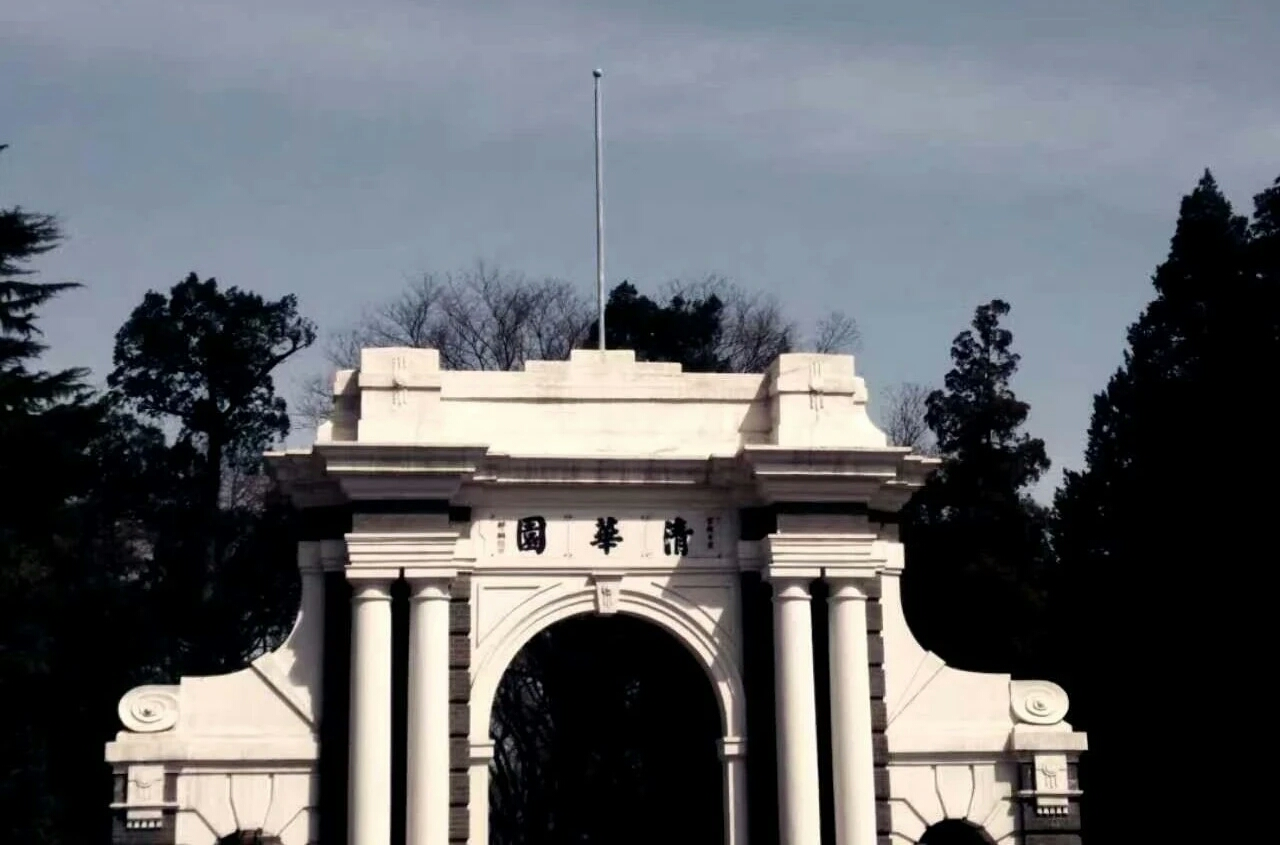
\includegraphics[width=\linewidth]{figures/二校门.jpg}
	清华园
\end{figure}

\paragraph{记事}
2020年由于突发的疫情,在家里困了一个学期,6月份终于允许毕业生返校。
笔者毕业后就要去其他学校读博了,因此这本来是能够留在园子里的最后一个学期,只是如今仅剩下寥寥的数周了。
此番离去,之后回来的机会便少了许多。为了能够多留下些回忆,笔者约了朋友C君再在最后离校前逛一逛清华园。
晚上走在人迹罕至的小路上,就会有一种微妙的紧张与刺激感,于是便和C君聊起了魑魅魍魉、月黑风高的事情,谈笑间产生了杜撰些怪谈的想法。
笔者文笔枯燥乏力,实在缺乏表现力,本来只当个玩笑,但终于还是决定写下来,权做四年清华生活的纪念。
此间故事,皆为杜撰;怪力乱神,洵有其缘;茶余闲谈,供君一笑耳。

% 简要提纲
% 
% 1. 素材
%    * 荷塘南面,西湖西北,小山上,月黑杀人夜,风高放火天,零零阁;亲历
%    * 荷塘仿若小提琴声的荷香,荷仙的歌声,荷塘月色;传说
%    * 装满水的西湖,服务看不见的客人;亲历
%    * 夜晚的工字厅,门口的灯,冥府之门;亲历+C君
%    * 二教的地下室,不开放自习,旧人体实验室;传说
%    * 大礼堂后的小径,限时开放,大礼堂的地下室;亲历+O君;引出O君,引出结界
%    * 荷塘东侧的小山,发现了蝠仙和蟾仙;O君带我们游历结界,讲解历史
%    * 苏世民书院后的凉风,正对的铜兽吐息,夏日冷若冰霜;和下面的可以凑一篇,最后O君带我们游历古战场,了解大战的历史
%    * 清芬园与苏世民之间的宿舍楼墙外隐约可见的字迹(毛主席的“人不犯我,我不犯人;人若犯我,我必犯人”)
% 2. 剧情与设定
%    * 零零阁引出无头杀人案
%    * 无头杀人案由荷仙引起
%    * 西湖服务看不见的客人
%    * 看不见的客人自工字厅的冥府之门而来
%    * 冥府收留了二教的孤魂野鬼
%    * 老建筑区有结界,保护着冥府不被外来的鬼蜮侵扰,结界定时打开,与外界通有无,通道即是大礼堂后限时开放的小径
%    * 结界的阵眼即在荷塘东侧的小山(毫无存在感),同时也是结界预留的逃生暗道,一旦礼堂后的门户被破坏,结界内的住民可通过此处快速逃生,不至于沦为瓮中之鳖
%    * 苏世民书院后,是古战场,老建筑区的冥府之民曾和别处的鬼蜮与此大战,留下无数冤魂,这之后请来了灵兽镇魂,并修建了老建筑区的结界
%    * 从地理上讲,食堂在结界之外,不如改成“冥界英雄纪念碑”,纪念大战中牺牲的冥府战士(我觉得很可)
% 3. 记事
%    * 6月23日,走了遍主楼后、综体前的小树林,看到了块灵璧石、五四广场,去游荷塘、寻零零阁,发现荷塘东南小山上的小乾坤,路过工字厅看到了门口开着的灯
%    * 7月7日,去了南园,观了“四院”(照澜院、新林院、普吉院、胜因院),找到了西南门和家园,细游荷塘东南的小山,黑暗中看了看苏世民书院后的铜鼎和铜兽
%    * 7月10日,绕文图,绕蒙民伟人文楼,路过再看了六教、校史馆、三教、四教,爬了旧水后的小丘,看了旧水、旧土、清华世纪鼎,看了新闻学院系馆,游了泥沙实验室后的“地质之角”,从历史楼旁经过,逛了结算中心南、西南联大纪念碑东的草丘,重观了清芬后五号楼上已褪色的大字,别后独游了原闻馨园北侧、苏世民书院后的几个老楼前新修的景观与花坛
%    * 7月13日,重游主楼后小树林,揭秘蒙民伟人文楼,探访出土文献保护中心,沿观畴西侧路北行,至新物理馆施工现场,西行至集体澡堂,环绕生物医学馆,途径人环楼至清华附中南口,后绕回直抵路北尽头,进入发电小院绕行一周,临近西北门而不得出,后进入学生区沿校河抵快递点,经W楼后校园最北道路经气膜馆拐至最东侧小路,经留学生公寓至东北门结束;后面一路上基本是沿着学校的边界在逛,和校外近在咫尺,触手可及,却又远在天涯,身不能达。
